\begin{figure}[t]
\centering
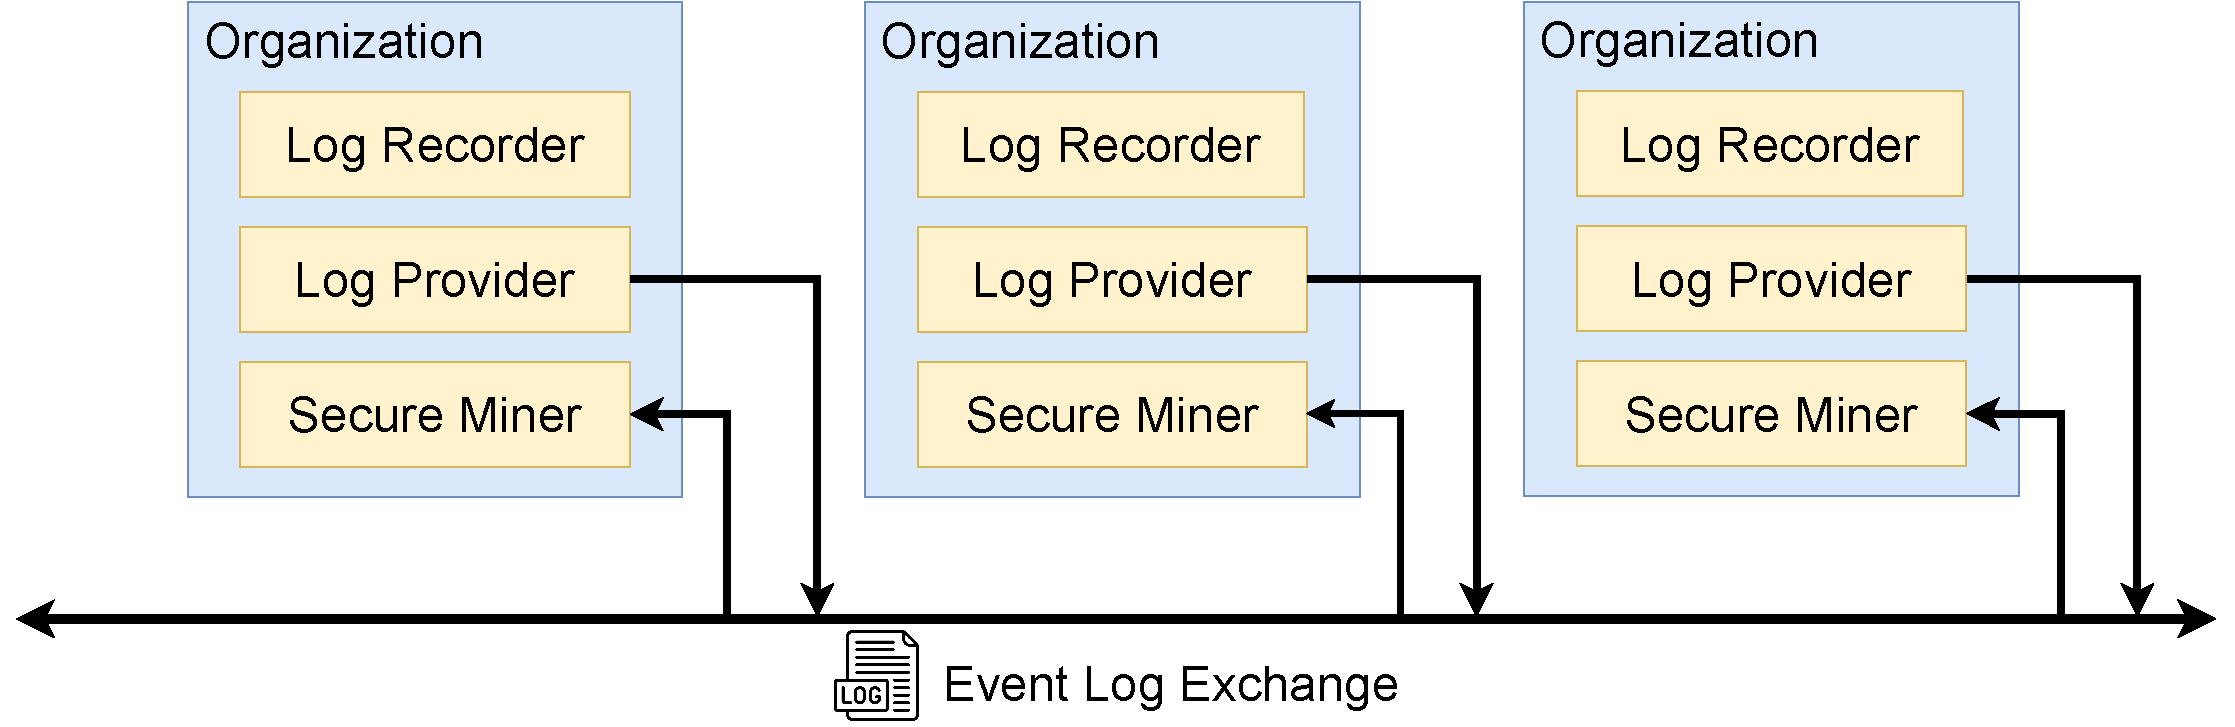
\includegraphics[width=0.9\linewidth]{content/figures/architecturediagram2.pdf}
\caption{High-level architectural overview.}
\label{fig:architecture_diagram}
\end{figure}
In this section, we present the high-level architecture underlying our solution. We consider the main functionalities of each component, avoiding details on the employed technologies discussed in the next sections. Once we introduced the architecture, we focus on the \Compo{Secure Miner} component that represents the core of our contribution.

\subsection{Architecture at large}
Our architecture involves different organizational ecosystems characterized by one or more machines. An \Compo{Organization} may assume one of the following two different roles or both: \textit{provisioner} if it delivers local event logs to be collaboratively mined; a \textit{miner} whenever it applies process mining algorithms using local event logs retrieved from provisioners. Provisioner \Compo{Organization}s collaborate to achieve common objectives and compose inter-organizational business processes whose event logs are scattered across multiple places. Each provisioner produces event logs, recording the operations executed to complete its part in the inter-organizational business process.  In \cref{fig:architecture_diagram}, we propose the high-level schematization of our solution. \Compo{Organization}s embed three main components, which we describe next: the \Compo{Log Recorder}, the \Compo{Log Provider}, and the \Compo{Secure Miner}. The maintenance of event logs is the core task performed by the \Compo{Log Recorder}. This component registers the events taking place in provisioner \Compo{Organization}s.  The \Actor{Hospital} and the other parties in our running example record Alice and Bob's traces using their \Compo{Log Recorder}s. The \Compo{Log Recorder} is queried by local \Compo{Log Providers} of the same \Compo{Organization} for event logs to be fed into remote \Compo{Secure Miner}s. The \Compo{Log Provider} component delivers on-demand data to \Compo{Secure Miner}s. It controls access to local event logs by authenticating data requests generated by miners. \Compo{Log Provider}s reject demands from unauthorized parties and only permit \texttt{Secure Miners} to use the data. In our motivating scenario, the \Actor{Specialized clinic}, \Actor{Pharmaceutical company}, and the \Actor{Hospital} leverage \Compo{Log Provider}s to authenticate the miner party before sending their logs. The \Compo{Secure Miner} shelters external event logs inside a miner ecosystem by preserving data confidentiality and integrity.  We provide an in-depth focus on the \Compo{Secure Miner} as follows.
\begin{figure}[t]
	\centering
	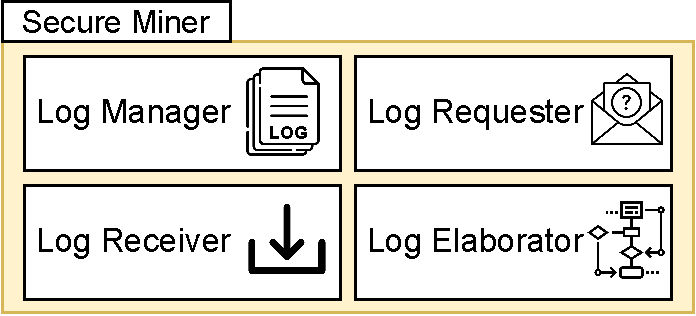
\includegraphics[width=0.5\linewidth]{content/figures/secureminer.pdf}
	\caption{Subcomponents of the Secure Miner.}
	\label{fig:trusted_miner}
\end{figure}
\subsection{Secure Miner}
The primary objective of the \Compo{Secure Miner} is to allow miners to securely execute process mining algorithms using event logs retrieved from provisioners such as the \Actor{Specialized clinic}, \Actor{Pharmaceutical company}, and the \Actor{Hospital} of our running example. \Compo{Secure Miner}s are isolated components that guarantee tamper-proofing and data confidentiality. In \cref{fig:trusted_miner}, we show a schematization of a \Compo{Secure Miner} in which we distinguish four different subcomponents: the \Compo{Log Manager}, the \Compo{Log Requester}, the \Compo{Log Receiver}, and the \Compo{Log Elaborator}. Event logs belonging to provisioners are locked in the \Compo{Secure Miner}. We handle these data via the \Compo{Log Manager} which prevents malicious parties from having direct access to event logs. These unauthorized entities include any component of the miner \Compo{Organization} outside the \Compo{Secure Miner}. Referring to our motivating scenario, the \Compo{Log Manager} of the miner isolates the traces of Alice and Bob from secrecy-attempting actions generated outside the \Compo{Secure Miner}. %Hence, it ensures the \Actor{Specialized clinic}, the \Actor{Hospital}, and the \Actor{Pharmaceutical company} that no entity of the miner access their traces, except for the secure subcomponents of the \Compo{Secure Miner}. 
The \Compo{Log Requester} and the \Compo{Log Receiver} are the subcomponents that we employ during the event log exchange. \Compo{Log Requester}s send authenticable data requests to the \Compo{Log Provider} component of provisioners. The \Compo{Log Receiver} collects event logs sent by \texttt{Log Providers} and entrusts them to the \Compo{Log Manager}. The miner of our motivating scenario employs these two components to retrieve the traces of Alice and Bob from the provisioners %owned by the \Actor{Specialized clinic} and the \Actor{Pharmaceutical company} 
and to collect this information in the \Compo{Secure Miner}. The \Compo{Log Elaborator} provides the functionality to securely execute process mining algorithms inside the \Compo{Secure Miner}. When activated, the \Compo{Log Elaborator} merge the traces locked in the \Compo{Secure Miner} in order to have a global view on the inter-organizational process comprensive of activities executed by each the party involved. Aggregated data is employeed by the \Compo{Log Elaborator} as input of process mining procedures. Mentioning our motivating scenario, the \Compo{Log Elaborator} combine the traces referring to the cases of Alice (i.e., $T^H_{312}$, $T^S_{312}$, and $T^C_{312}$) and Bob (i.e, $T^H_{711}$, $T^S_{711}$, and $T^C_{711}$ ) generating the chronologically sorted traces $T_{312}$ and $T_{711}$ to be fed into mining algorithms.  %that are generated by the \Actor{Specialized clinic}, \Actor{Pharmaceutical company} and subsequently apply the process discovery algorithm. fed into process mining algorithms



